\documentclass[11pt,a4paper]{article}
\usepackage[T1]{fontenc}
\usepackage[utf8]{inputenc}
\usepackage[magyar]{babel}
\usepackage{lmodern}
\usepackage{amsmath,amssymb}
\usepackage{enumitem}
\usepackage{array}
\usepackage{tikz}
\usetikzlibrary{decorations.markings,arrows.meta}
\usepackage[most]{tcolorbox}
\usepackage[a4paper,margin=1.8cm]{geometry}
\usepackage{needspace}

\pagestyle{empty}
\setlength{\parindent}{0pt}
\setlength{\parskip}{3pt}
\setlist{nosep,leftmargin=1.5em}

\tikzset{
  midarrow/.style={postaction={decorate},
    decoration={markings, mark=at position 0.55 with {\arrow{Stealth[length=2.5mm]}}}}
}

\newtcolorbox{kepletdoboz}[1]{colback=blue!3,colframe=blue!45!black,
  fonttitle=\bfseries,title=#1,left=4pt,right=4pt,top=3pt,bottom=3pt,
  before skip=6pt,after skip=6pt}
\newtcolorbox{figyelem}{colback=red!4,colframe=red!55!black,
  fonttitle=\bfseries,title=Gyakori hibák,left=4pt,right=4pt,top=3pt,bottom=3pt,
  before skip=6pt,after skip=6pt}

\newcommand{\szakasz}[1]{\par\Needspace{8\baselineskip}\medskip{\large\bfseries #1}\par\smallskip}

% kis diagram: #1 = x tengely, #2 = y tengely, #3 = görbe rajza
\newcommand{\minidiag}[3]{%
  \begin{tikzpicture}[scale=0.55,>=Stealth,baseline=(current bounding box.center)]
    \draw[->] (0,0) -- (2.6,0) node[below] {\scriptsize $#1$};
    \draw[->] (0,0) -- (0,2.3) node[left] {\scriptsize $#2$};
    #3
  \end{tikzpicture}}

\begin{document}

\begin{center}
  {\LARGE\bfseries Termodinamika -- összefoglaló}\\[4pt]
  {\small 2.--5.~óra: állapotjelzők, főtételek, körfolyamatok, hőerőgépek}
\end{center}

\begin{tcolorbox}[colback=yellow!8,colframe=orange!70!black,left=4pt,right=4pt,top=2pt,bottom=2pt]
\centering
Végig a $\Delta E = Q + W$ alakot használjuk, ahol $W$ a \textbf{gázon végzett} munka.
Hőmérséklettel mindig \textbf{kelvinben} számolunk: $T\,[\text{K}] = t\,[^\circ\text{C}] + 273$.
\end{tcolorbox}

%--------------------------------------------------------------------
\szakasz{1. Alapfogalmak}

\begin{itemize}
  \item \textbf{Állapotjelzők:} a rendszer pillanatnyi állapotát írják le, csak a
    kezdő- és végállapottól függenek, az úttól nem: $p$, $V$, $T$, $n$, és a
    \textbf{belső energia} ($E$).
  \item \textbf{Folyamatjellemzők:} csak egy folyamat \emph{közben} értelmezhetők, és függenek
    attól, milyen úton jut el a rendszer egyik állapotból a másikba: a \textbf{hő} ($Q$) és a
    \textbf{munka} ($W$). ,,A gáznak van hője'' -- ez hibás mondat; a gáznak belső energiája
    van, hőt csak \emph{felvenni} vagy \emph{leadni} lehet.
  \item \textbf{Belső energia:} a részecskék mozgási (és kölcsönhatási) energiáinak összege.
    Ideális gázban nincs kölcsönhatás, ezért $E$ \textbf{csak a hőmérséklettől} függ.
  \item \textbf{Hő:} a hőmérséklet-különbség miatt, rendezetlen módon átadott energia.
    \textbf{Munka:} rendezett módon (pl.\ dugattyú elmozdulásával) átadott energia.
\end{itemize}

%--------------------------------------------------------------------
\szakasz{2. Az ideális gáz}

\begin{kepletdoboz}{Állapotegyenlet és belső energia}
\begin{minipage}[t]{0.5\linewidth}
\[ pV = nRT = NkT \]
\[ \frac{p_1V_1}{T_1} = \frac{p_2V_2}{T_2} \quad (\text{zárt gázra}) \]
\end{minipage}\hfill
\begin{minipage}[t]{0.48\linewidth}
\[ E = \frac{f}{2}\,nRT, \qquad \Delta E = \frac{f}{2}\,nR\,\Delta T = n\,c_V\,\Delta T \]
\end{minipage}

\smallskip
$R = 8{,}31~\tfrac{\text{J}}{\text{mol}\cdot\text{K}}$, $\;k = 1{,}38\cdot 10^{-23}~\tfrac{\text{J}}{\text{K}}$,
$\;N_A = 6\cdot 10^{23}~\tfrac{1}{\text{mol}}$.
Szabadsági fokok: egyatomos gáz $f = 3$, kétatomos gáz $f = 5$.\\
Hasznos átírás: $nR\,\Delta T = \Delta(pV)$, így pl.\ egyatomos gázra
$\Delta E = \tfrac32\,\Delta(pV)$.
\end{kepletdoboz}

%--------------------------------------------------------------------
\szakasz{3. Munka a $p$--$V$ diagramon}

\begin{minipage}[t]{0.58\linewidth}\vspace{0pt}
\begin{itemize}
  \item Állandó nyomáson: $\;W = -p\,\Delta V$.
  \item Általában: $|W|$ a $p$--$V$ görbe \textbf{alatti terület}.
  \item \textbf{Előjel:} összenyomás ($\Delta V < 0$) $\Rightarrow W > 0$ (mi végzünk
    munkát a gázon); tágulás ($\Delta V > 0$) $\Rightarrow W < 0$ (a gáz végez munkát).
  \item Izochor folyamatban $W = 0$.
  \item A munka függ az úttól: ugyanazon két állapot között más görbe alatt más a
    terület.
\end{itemize}
\end{minipage}\hfill
\begin{minipage}[t]{0.38\linewidth}\vspace{0pt}\centering
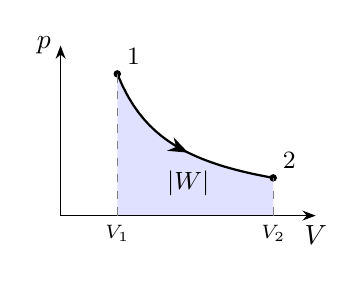
\begin{tikzpicture}[scale=0.9,>=Stealth]
  \fill[blue!12] (0.8,0) -- plot[domain=0.8:3,samples=30] (\x,{1.6/\x}) -- (3,0) -- cycle;
  \draw[->] (0,0) -- (3.6,0) node[below] {$V$};
  \draw[->] (0,0) -- (0,2.4) node[left] {$p$};
  \draw[thick,midarrow,domain=0.8:3,samples=30] plot (\x,{1.6/\x});
  \fill (0.8,2) circle (1.5pt) node[above right] {\small 1};
  \fill (3,0.533) circle (1.5pt) node[above right] {\small 2};
  \draw[gray,dashed] (0.8,0) node[below,black] {\scriptsize $V_1$} -- (0.8,2);
  \draw[gray,dashed] (3,0) node[below,black] {\scriptsize $V_2$} -- (3,0.533);
  \node at (1.8,0.45) {\small $|W|$};
\end{tikzpicture}
\end{minipage}

%--------------------------------------------------------------------
\szakasz{4. A hőtan I.~főtétele}

\begin{kepletdoboz}{I.~főtétel (energiamegmaradás)}
\[ \Delta E = Q + W \]
\begin{tabular}{@{}ll@{}}
$Q > 0$: a gáz hőt \textbf{vesz fel}; & $Q < 0$: a gáz hőt \textbf{ad le}; \\
$W > 0$: \textbf{mi végzünk} munkát a gázon (összenyomás); &
$W < 0$: \textbf{a gáz végez} munkát (tágulás).
\end{tabular}
\end{kepletdoboz}
{\small\emph{Vigyázat:} sok tankönyv a gáz által végzett munkával írja fel:
$Q = \Delta E + W_\text{gáz}$. A kettő ugyanazt mondja, csak $W_\text{gáz} = -W$.}

%--------------------------------------------------------------------
\szakasz{5. Speciális állapotváltozások}

\begin{center}
\renewcommand{\arraystretch}{1.55}
\begin{tabular}{|l|c|c|c|c|c|}
\hline
\textbf{Folyamat} & \textbf{Feltétel} & \textbf{Gáztörvény} & $\boldsymbol{W}$ & $\boldsymbol{Q}$ & $\boldsymbol{\Delta E}$ \\ \hline
izochor   & $V$ = áll. & $p/T$ = áll. & $0$ & $n\,c_V\,\Delta T$ & $Q$ \\ \hline
izobár    & $p$ = áll. & $V/T$ = áll. & $-p\,\Delta V = -nR\,\Delta T$ & $n\,c_p\,\Delta T$ & $n\,c_V\,\Delta T$ \\ \hline
izoterm   & $T$ = áll. & $pV$ = áll.  & $-Q$ (terület) & $-W$ & $0$ \\ \hline
adiabatikus & $Q = 0$ & $pV^\kappa$ = áll.$^*$ & $\Delta E$ & $0$ & $n\,c_V\,\Delta T$ \\ \hline
\end{tabular}

\smallskip
{\small $^*$\,$\kappa = c_p/c_V$ (egyatomos gázra $5/3$). Számolni nem kell vele, de innen
látszik, hogy az adiabata \emph{meredekebb}, mint az izoterma.}
\end{center}

\begin{minipage}[t]{0.40\linewidth}\vspace{0pt}\centering
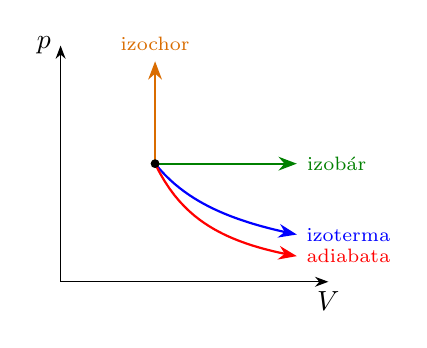
\begin{tikzpicture}[scale=1.0,>=Stealth]
  \draw[->] (0,0) -- (3.4,0) node[below] {$V$};
  \draw[->] (0,0) -- (0,3.0) node[left] {$p$};
  \draw[thick,green!50!black,->] (1.2,1.5) -- (3.0,1.5) node[right] {\scriptsize izobár};
  \draw[thick,orange!85!black,->] (1.2,1.5) -- (1.2,2.8) node[above] {\scriptsize izochor};
  \draw[thick,blue,->,domain=1.2:3.0,samples=30] plot (\x,{1.8/\x});
  \node[blue,right] at (3.0,0.6) {\scriptsize izoterma};
  \draw[thick,red,->,domain=1.2:3.0,samples=30] plot (\x,{1.5*(1.2/\x)^1.667});
  \node[red,right] at (3.0,0.33) {\scriptsize adiabata};
  \fill (1.2,1.5) circle (1.6pt);
\end{tikzpicture}\\
{\small Tágulások közös kezdőpontból}
\end{minipage}\hfill
\begin{minipage}[t]{0.57\linewidth}\vspace{0pt}
\begin{itemize}
  \item \textbf{Izoterm folyamatban is van hőcsere!} Tágulásnál a gáz annyi hőt vesz fel,
    amennyi munkát végez ($\Delta E = 0$).
  \item \textbf{Adiabatikus:} nincs hőcsere. Jó közelítéssel ilyen minden \emph{gyors}
    folyamat, mert a hővezetéshez idő kell (biciklipumpa, dezodoros flakon, motor
    hengere). Összenyomáskor a gáz \emph{felmelegszik}, táguláskor \emph{lehűl}.
  \item Ugyanabból a pontból indulva az adiabata összenyomáskor az izoterma
    \emph{fölött}, táguláskor \emph{alatta} halad.
\end{itemize}
\end{minipage}

\medskip
\textbf{A három ,,klasszikus'' folyamat a három diagramtípuson}
(nyíl: melegítés/tágulás iránya):

\begin{center}
\renewcommand{\arraystretch}{1.1}
\begin{tabular}{>{\bfseries}l c c c}
 & $p$--$V$ & $V$--$T$ & $p$--$T$ \\[2pt]
izobár &
\minidiag{V}{p}{\draw[thick,->] (0.6,1.3) -- (2.1,1.3);} &
\minidiag{T}{V}{\draw[gray,dashed] (0,0) -- (0.6,0.5); \draw[thick,->] (0.6,0.5) -- (2.1,1.75);} &
\minidiag{T}{p}{\draw[thick,->] (0.6,1.3) -- (2.1,1.3);} \\
izochor &
\minidiag{V}{p}{\draw[thick,->] (1.2,0.5) -- (1.2,1.9);} &
\minidiag{T}{V}{\draw[thick,->] (0.6,1.2) -- (2.1,1.2);} &
\minidiag{T}{p}{\draw[gray,dashed] (0,0) -- (0.6,0.5); \draw[thick,->] (0.6,0.5) -- (2.1,1.75);} \\
izoterm &
\minidiag{V}{p}{\draw[thick,->,domain=0.6:2.2,samples=25] plot (\x,{1.0/\x});} &
\minidiag{T}{V}{\draw[thick,->] (1.2,0.5) -- (1.2,1.9);} &
\minidiag{T}{p}{\draw[thick,<-] (1.2,0.5) -- (1.2,1.9);} \\
\end{tabular}
\end{center}
{\small Az origón átmenő egyenes azt jelenti, hogy a két mennyiség egyenesen arányos.
Az izoterm tágulásnál $V$ nő, $p$ csökken.}

%--------------------------------------------------------------------
\szakasz{6. Fajhő, mólhő, halmazállapot-változás}

\begin{kepletdoboz}{Hőközlés}
\begin{minipage}[t]{0.62\linewidth}
\textbf{Melegítés (szilárd, folyadék):} $\;Q = c\,m\,\Delta T$\\
\textbf{Gázok, mólhővel:} $\;Q_V = n\,c_V\,\Delta T$, $\quad Q_p = n\,c_p\,\Delta T$\\
\textbf{Mayer-egyenlet:} $\;c_p - c_V = R$
\end{minipage}\hfill
\begin{minipage}[t]{0.35\linewidth}\vspace{-8pt}
\renewcommand{\arraystretch}{1.25}
\begin{tabular}{|l|c|c|}
\hline
 & $c_V$ & $c_p$ \\ \hline
egyatomos gáz & $\tfrac32 R$ & $\tfrac52 R$ \\
kétatomos gáz & $\tfrac52 R$ & $\tfrac72 R$ \\ \hline
\end{tabular}
\end{minipage}

\smallskip
\textbf{Halmazállapot-változás:} $\;Q = L\,m$ (olvadáshő $L_\text{o}$, forráshő $L_\text{f}$),
közben a hőmérséklet \textbf{állandó}.\\
Víz: $c = 4180~\tfrac{\text{J}}{\text{kg}\cdot\text{K}}$,
$\;L_\text{o} = 334~\tfrac{\text{kJ}}{\text{kg}}$,
$\;L_\text{f} = 2256~\tfrac{\text{kJ}}{\text{kg}}$.
\end{kepletdoboz}

\begin{minipage}[t]{0.58\linewidth}\vspace{0pt}
\begin{itemize}
  \item \textbf{Miért $c_p > c_V$?} Ugyanakkora $\Delta T$-hez ugyanakkora $\Delta E$ tartozik.
    Állandó nyomáson a gáz közben ki is tágul és munkát végez, ezért ennyivel
    ($p\Delta V = nR\Delta T$) több hőt kell közölni.
  \item \textbf{Olvadás, forrás közben} a közölt hő a részecskék közötti kötések
    felbontására fordítódik: a belső energia \emph{nő}, de a hőmérséklet nem változik.
    (Itt nem ideális gázról van szó, ezért $E$ nem csak $T$-től függ.)
\end{itemize}
\end{minipage}\hfill
\begin{minipage}[t]{0.38\linewidth}\vspace{0pt}\centering
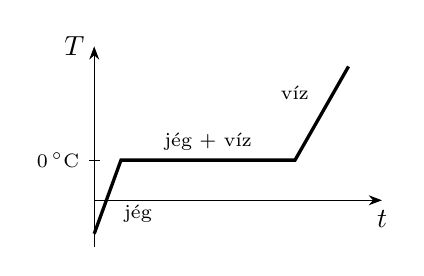
\begin{tikzpicture}[scale=0.85,>=Stealth]
  \draw[->] (0,0) -- (4.3,0) node[below] {$t$};
  \draw[->] (0,-0.7) -- (0,2.3) node[left] {$T$};
  \draw (0.08,0.6) -- (-0.08,0.6) node[left] {\scriptsize $0\,^\circ$C};
  \draw[very thick] (0,-0.5) -- (0.4,0.6) -- (3.0,0.6) -- (3.8,2.0);
  \node[above] at (1.7,0.6) {\scriptsize jég + víz};
  \node[right] at (0.3,-0.2) {\scriptsize jég};
  \node[left] at (3.35,1.6) {\scriptsize víz};
\end{tikzpicture}\\
{\small Melegítés állandó teljesítménnyel}
\end{minipage}

%--------------------------------------------------------------------
\szakasz{7. Körfolyamatok}

\begin{minipage}[t]{0.58\linewidth}\vspace{0pt}
\begin{itemize}
  \item A gáz visszatér a kiinduló állapotba, ezért \textbf{$\Delta E_\text{össz} = 0$}
    (az állapotjelzők mind visszaállnak).
  \item Az I.~főtételből: $Q_\text{össz} = -W_\text{össz}$, azaz
    $Q_\text{fel} - |Q_\text{le}| = W_\text{h}$.
  \item A hasznos munka nagysága a görbe által \textbf{bezárt terület}.
  \item \textbf{Körüljárási irány:}
    \begin{itemize}
      \item óramutató járásával \textbf{megegyező} $\Rightarrow$ a gáz végez munkát:
        \textbf{hőerőgép};
      \item óramutató járásával \textbf{ellentétes} $\Rightarrow$ mi végzünk munkát:
        \textbf{hűtőgép / hőszivattyú}.
    \end{itemize}
  \item Fordított irányban minden szakaszon megfordul $Q$, $W$ és $\Delta E$ előjele.
  \item \textbf{Számolási recept:} 1) $T$ minden csúcsban ($pV = nRT$);
    2) szakaszonként $W$ (terület), $\Delta E$ ($\tfrac f2\,\Delta(pV)$), $Q = \Delta E - W$;
    3) ellenőrzés: $\sum \Delta E = 0$, $\sum Q = -\sum W$.
\end{itemize}
\end{minipage}\hfill
\begin{minipage}[t]{0.38\linewidth}\vspace{0pt}\centering
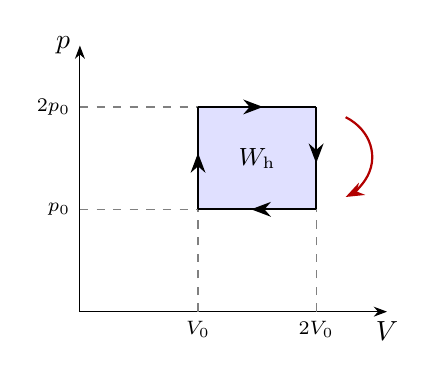
\begin{tikzpicture}[x=1.5cm,y=1.3cm,>=Stealth]
  \fill[blue!12] (1,1) rectangle (2,2);
  \draw[->] (0,0) -- (2.6,0) node[below] {$V$};
  \draw[->] (0,0) -- (0,2.6) node[left] {$p$};
  \draw[dashed,gray] (1,0) node[below,black] {\scriptsize $V_0$} -- (1,1);
  \draw[dashed,gray] (2,0) node[below,black] {\scriptsize $2V_0$} -- (2,1);
  \draw[dashed,gray] (0,1) node[left,black] {\scriptsize $p_0$} -- (1,1);
  \draw[dashed,gray] (0,2) node[left,black] {\scriptsize $2p_0$} -- (1,2);
  \draw[thick,midarrow] (1,1) -- (1,2);
  \draw[thick,midarrow] (1,2) -- (2,2);
  \draw[thick,midarrow] (2,2) -- (2,1);
  \draw[thick,midarrow] (2,1) -- (1,1);
  \node at (1.5,1.5) {\small $W_\text{h}$};
  \draw[->,thick,red!70!black] (2.25,1.9) arc (60:-60:0.45);
\end{tikzpicture}\\
{\small Óramutató járásával megegyező: hőerőgép (4.~óra)}
\end{minipage}

%--------------------------------------------------------------------
\szakasz{8. Hőerőgép, hűtőgép, hőszivattyú}

\begin{center}
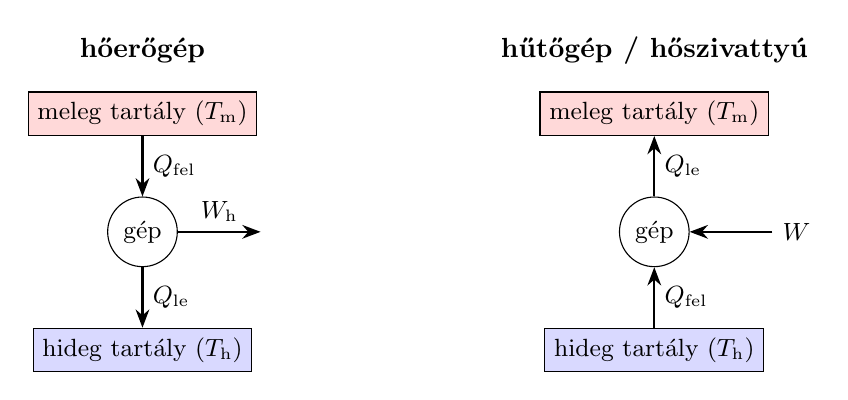
\begin{tikzpicture}[font=\small]
  \begin{scope}
    \node[draw,fill=red!15,minimum width=2.6cm,minimum height=0.55cm] (M) at (0,1.5) {meleg tartály ($T_\text{m}$)};
    \node[draw,circle,minimum size=0.8cm] (G) at (0,0) {gép};
    \node[draw,fill=blue!15,minimum width=2.6cm,minimum height=0.55cm] (H) at (0,-1.5) {hideg tartály ($T_\text{h}$)};
    \draw[-{Stealth},thick] (M) -- node[right] {$Q_\text{fel}$} (G);
    \draw[-{Stealth},thick] (G) -- node[right] {$Q_\text{le}$} (H);
    \draw[-{Stealth},thick] (G) -- node[above] {$W_\text{h}$} (1.5,0);
    \node[font=\bfseries] at (0,2.3) {hőerőgép};
  \end{scope}
  \begin{scope}[xshift=6.5cm]
    \node[draw,fill=red!15,minimum width=2.6cm,minimum height=0.55cm] (M) at (0,1.5) {meleg tartály ($T_\text{m}$)};
    \node[draw,circle,minimum size=0.8cm] (G) at (0,0) {gép};
    \node[draw,fill=blue!15,minimum width=2.6cm,minimum height=0.55cm] (H) at (0,-1.5) {hideg tartály ($T_\text{h}$)};
    \draw[-{Stealth},thick] (G) -- node[right] {$Q_\text{le}$} (M);
    \draw[-{Stealth},thick] (H) -- node[right] {$Q_\text{fel}$} (G);
    \draw[-{Stealth},thick] (1.5,0) node[right] {$W$} -- (G);
    \node[font=\bfseries] at (0,2.3) {hűtőgép / hőszivattyú};
  \end{scope}
\end{tikzpicture}
\end{center}

\begin{kepletdoboz}{Hatásfok és jósági tényező}
\begin{minipage}[t]{0.48\linewidth}
\textbf{Hőerőgép} ($W_\text{h} = Q_\text{fel} - |Q_\text{le}|$):
\[ \eta = \frac{W_\text{h}}{Q_\text{fel}} = 1 - \frac{|Q_\text{le}|}{Q_\text{fel}}
   \;\le\; 1 - \frac{T_\text{h}}{T_\text{m}} \]
A nevezőben \textbf{csak a felvett hő} áll!
\end{minipage}\hfill
\begin{minipage}[t]{0.48\linewidth}
\textbf{Hűtőgép, hőszivattyú} ($|Q_\text{le}| = Q_\text{fel} + W$):
\[ \varepsilon_\text{hűtő} = \frac{Q_\text{fel}}{W} \le \frac{T_\text{h}}{T_\text{m}-T_\text{h}} \]
\[ \varepsilon_\text{fűtő} = \frac{|Q_\text{le}|}{W} \le \frac{T_\text{m}}{T_\text{m}-T_\text{h}} \]
Lehet $1$-nél nagyobb, ez nem sérti az energiamegmaradást.
\end{minipage}

\smallskip
A felső korlátok a \emph{két tartály} között működő ideális (Carnot-) gépre vonatkoznak;
a valódi gépek ennél mindig rosszabbak. Ha egy körfolyamatban sokféle hőmérsékleten
történik hőcsere, a korlát csak a legmagasabb és a legalacsonyabb hőmérséklettel
becsülhető.
\end{kepletdoboz}

%--------------------------------------------------------------------
\szakasz{9. A hőtan II.~főtétele}

\begin{kepletdoboz}{II.~főtétel -- két egyenértékű megfogalmazás}
\begin{itemize}
  \item \textbf{Clausius:} a hő magától mindig a melegebb testről a hidegebbre áramlik,
    fordítva csak külső munka árán (hűtőgép).
  \item \textbf{Kelvin--Planck:} nincs olyan periodikusan működő gép, amely egyetlen
    tartályból felvett hőt \emph{teljes egészében} munkává alakítana. Kell hideg tartály
    is, ezért $\eta < 1$.
\end{itemize}
A természetes folyamatok \textbf{irreverzibilisek} (megfordíthatatlanok): magától a
rendezetlenség növekedése felé haladnak (kávé kihűl, labda pattogása abbamarad,
gázok keverednek), visszafelé nem.
\end{kepletdoboz}

\begin{center}
\renewcommand{\arraystretch}{1.4}
\newcolumntype{R}[1]{>{\raggedright\arraybackslash}p{#1}}
\begin{tabular}{|R{2.9cm}|R{5.6cm}|R{2.7cm}|R{3.7cm}|}
\hline
 & \textbf{Mit csinálna?} & \textbf{Melyik főtételt sérti?} & \textbf{Példa} \\ \hline
\textbf{Elsőfajú perpetuum mobile} & energiabefektetés nélkül végezne munkát
  (a semmiből termelne energiát) & I.~főtétel & ,,önhajtó'' kerék, motor + generátor kör \\ \hline
\textbf{Másodfajú perpetuum mobile} & egyetlen tartály hőjét alakítaná teljesen
  munkává (energia megmarad!) & II.~főtétel & a tenger hőjéből hajtott hajó \\ \hline
\end{tabular}
\end{center}
{\small Két különböző hőmérsékletű tartály között már lehet munkát nyerni (pl.\ meleg
felszíni és hideg mélységi tengervíz között), de csak $\eta \le 1 - T_\text{h}/T_\text{m}$
hatásfokkal.}

%--------------------------------------------------------------------
\begin{figyelem}
\begin{itemize}
  \item Celsius-fokban számolni a gáztörvényekben vagy a hatásfok-korlátban
    ($1 - 5/25 \neq 1 - 278/298$).
  \item Előjelhiba a munkánál: összenyomáskor $W > 0$, tágulásnál $W < 0$.
  \item ,,Hőközléskor mindig nő a hőmérséklet'' -- nem: izoterm tágulás, olvadás.
  \item ,,Adiabatikus $=$ állandó hőmérsékletű'' -- nem: adiabatikusnál $Q = 0$, a
    hőmérséklet változik.
  \item Körfolyamatban $\Delta E = 0$, de $Q_\text{össz}$ és $W_\text{össz}$ \emph{nem} nulla
    (a hurok területe).
  \item A hatásfok nevezőjébe a hők előjeles összege kerül -- így mindig $100\%$ jönne ki.
  \item ,,A hőszivattyú 400\%-os hatásfokkal működik, tehát sérti az energiamegmaradást''
    -- nem: a többlethőt a hideg környezetből szivattyúzza át.
\end{itemize}
\end{figyelem}

\end{document}
